\documentclass[a4paper]{report}
\author{Jure Kos}
\title{Vaja 20, Prožnostni modul}
\date{2.1.2022}
\usepackage{graphicx}
\graphicspath{ {./images/} }

\begin{document}

\maketitle

\chapter*{Uvod}
Pri majhni deformaciji telesa je sila, ki deformacijo povzroči, sorazmerna z deformacijo (Hookov zakon). Pri ravni žici je relativni raztezek $\Delta l/l$ sorazmeren z natezno napetostjo $F/S$:

\[\Delta l/l = (1/E)(F/S)\]

Pri tem je E prožnostni modul snovi. Vrednost E je za večino kovin okrog $10^7$ $N/cm^2$.\\
Natezno napetost, pri kateri Hookov zakon neha veljati, imenujemo mejo linearnosti. Natezno napetost, pri kateri se snov že deformira pa imenujemo meja prožnosti. Ta je za kovine nekajkrat $10^4$ $N/cm^2$.\\ Ce prekoračimo to mejo, se žica po razbremenitvi ne skrči več na svojo prvotno dolžino, ampak ohrani trajen podaljšek. Če obremenjujemo žico še naprej, prekoračimo končno tudi mejo trdnosti in žica se pretrga.

\section{Naloga}
Določiti prožnostni modul, mejo linearnosti in mejo natezne trdnosti za bakreno žico in prožnostni modul jeklene žice.

\section{Potrebščine}
1. Mizica z merili, privitimi na zid,\\
2. merjenec (bakrena in jeklena žica),\\
3. uteži s kljukicami,\\
4. mikrometerski vijak.
\chapter*{Potek}
Izmerimo premer žice na več mestih z mikrometrom in odberimo dolžino žice! Nato obesimo utež 150 g, zato da se žica izravna in zapišemo začetno lego $x_0$. Sedaj žico postopoma  obremenjujemo in si vsakič odberemo lego $x$ z natančnostjo odčitka na noniju. Vse podatke vnašamo v tabelo.\\
Med meritvijo sproti izračunavamo zaporedne podaljške $\Delta x=x_n -x_{n-1}$. Ko začno podaljški naraščati, smo prekoračili mejo linearnosti. Tedaj postopoma razbremenjujemo žico in podobno kot prej izmerimo vse količine. Če ostane žica po razbremenitvi deformirana, je bila prekoračena tudi meja prožnosti. 
Mejo natezne trdnosti določimo tako, da obesimo kratko bakreno žico z znanim presekom na kavelj in jo postopoma obremenjujemo z utežmi, dokler se ne pretrga. Tudi to meritev večkrat ponovimo.
Prožnostni modul določimo grafično iz narisanega diagrama. Kot abscise nanašamo razlike napetosti $(F-F_0)/S$ kot ordinate pa relativne raztezke $\Delta l/l$. Med točkami, ki jih tako dobiš, potegni na oko najboljšo premico. Strmina dobljene premice je $1/E$ (glej enačbo). Iz diagrama za bakreno žico oceniš se mejo linearnosti. Ko prekoračimo to mejo, zveza med nateznim tlakom in relativnim raztezkom ni več linearna - raztezki so tedaj večji, kot bi bili po Hookovem zakonu. Krivulja $\Delta l/l = f(F -F_0)/S$ postane bolj strma kot premica $\Delta l/l =(1/E) (F -F_0)/S $.

\chapter*{Meritve}
Debeline žic smo izmerili kot 0,28mm za jekleno in 0,35mm za bakreno.

Raztezke smo izmerili kot\\
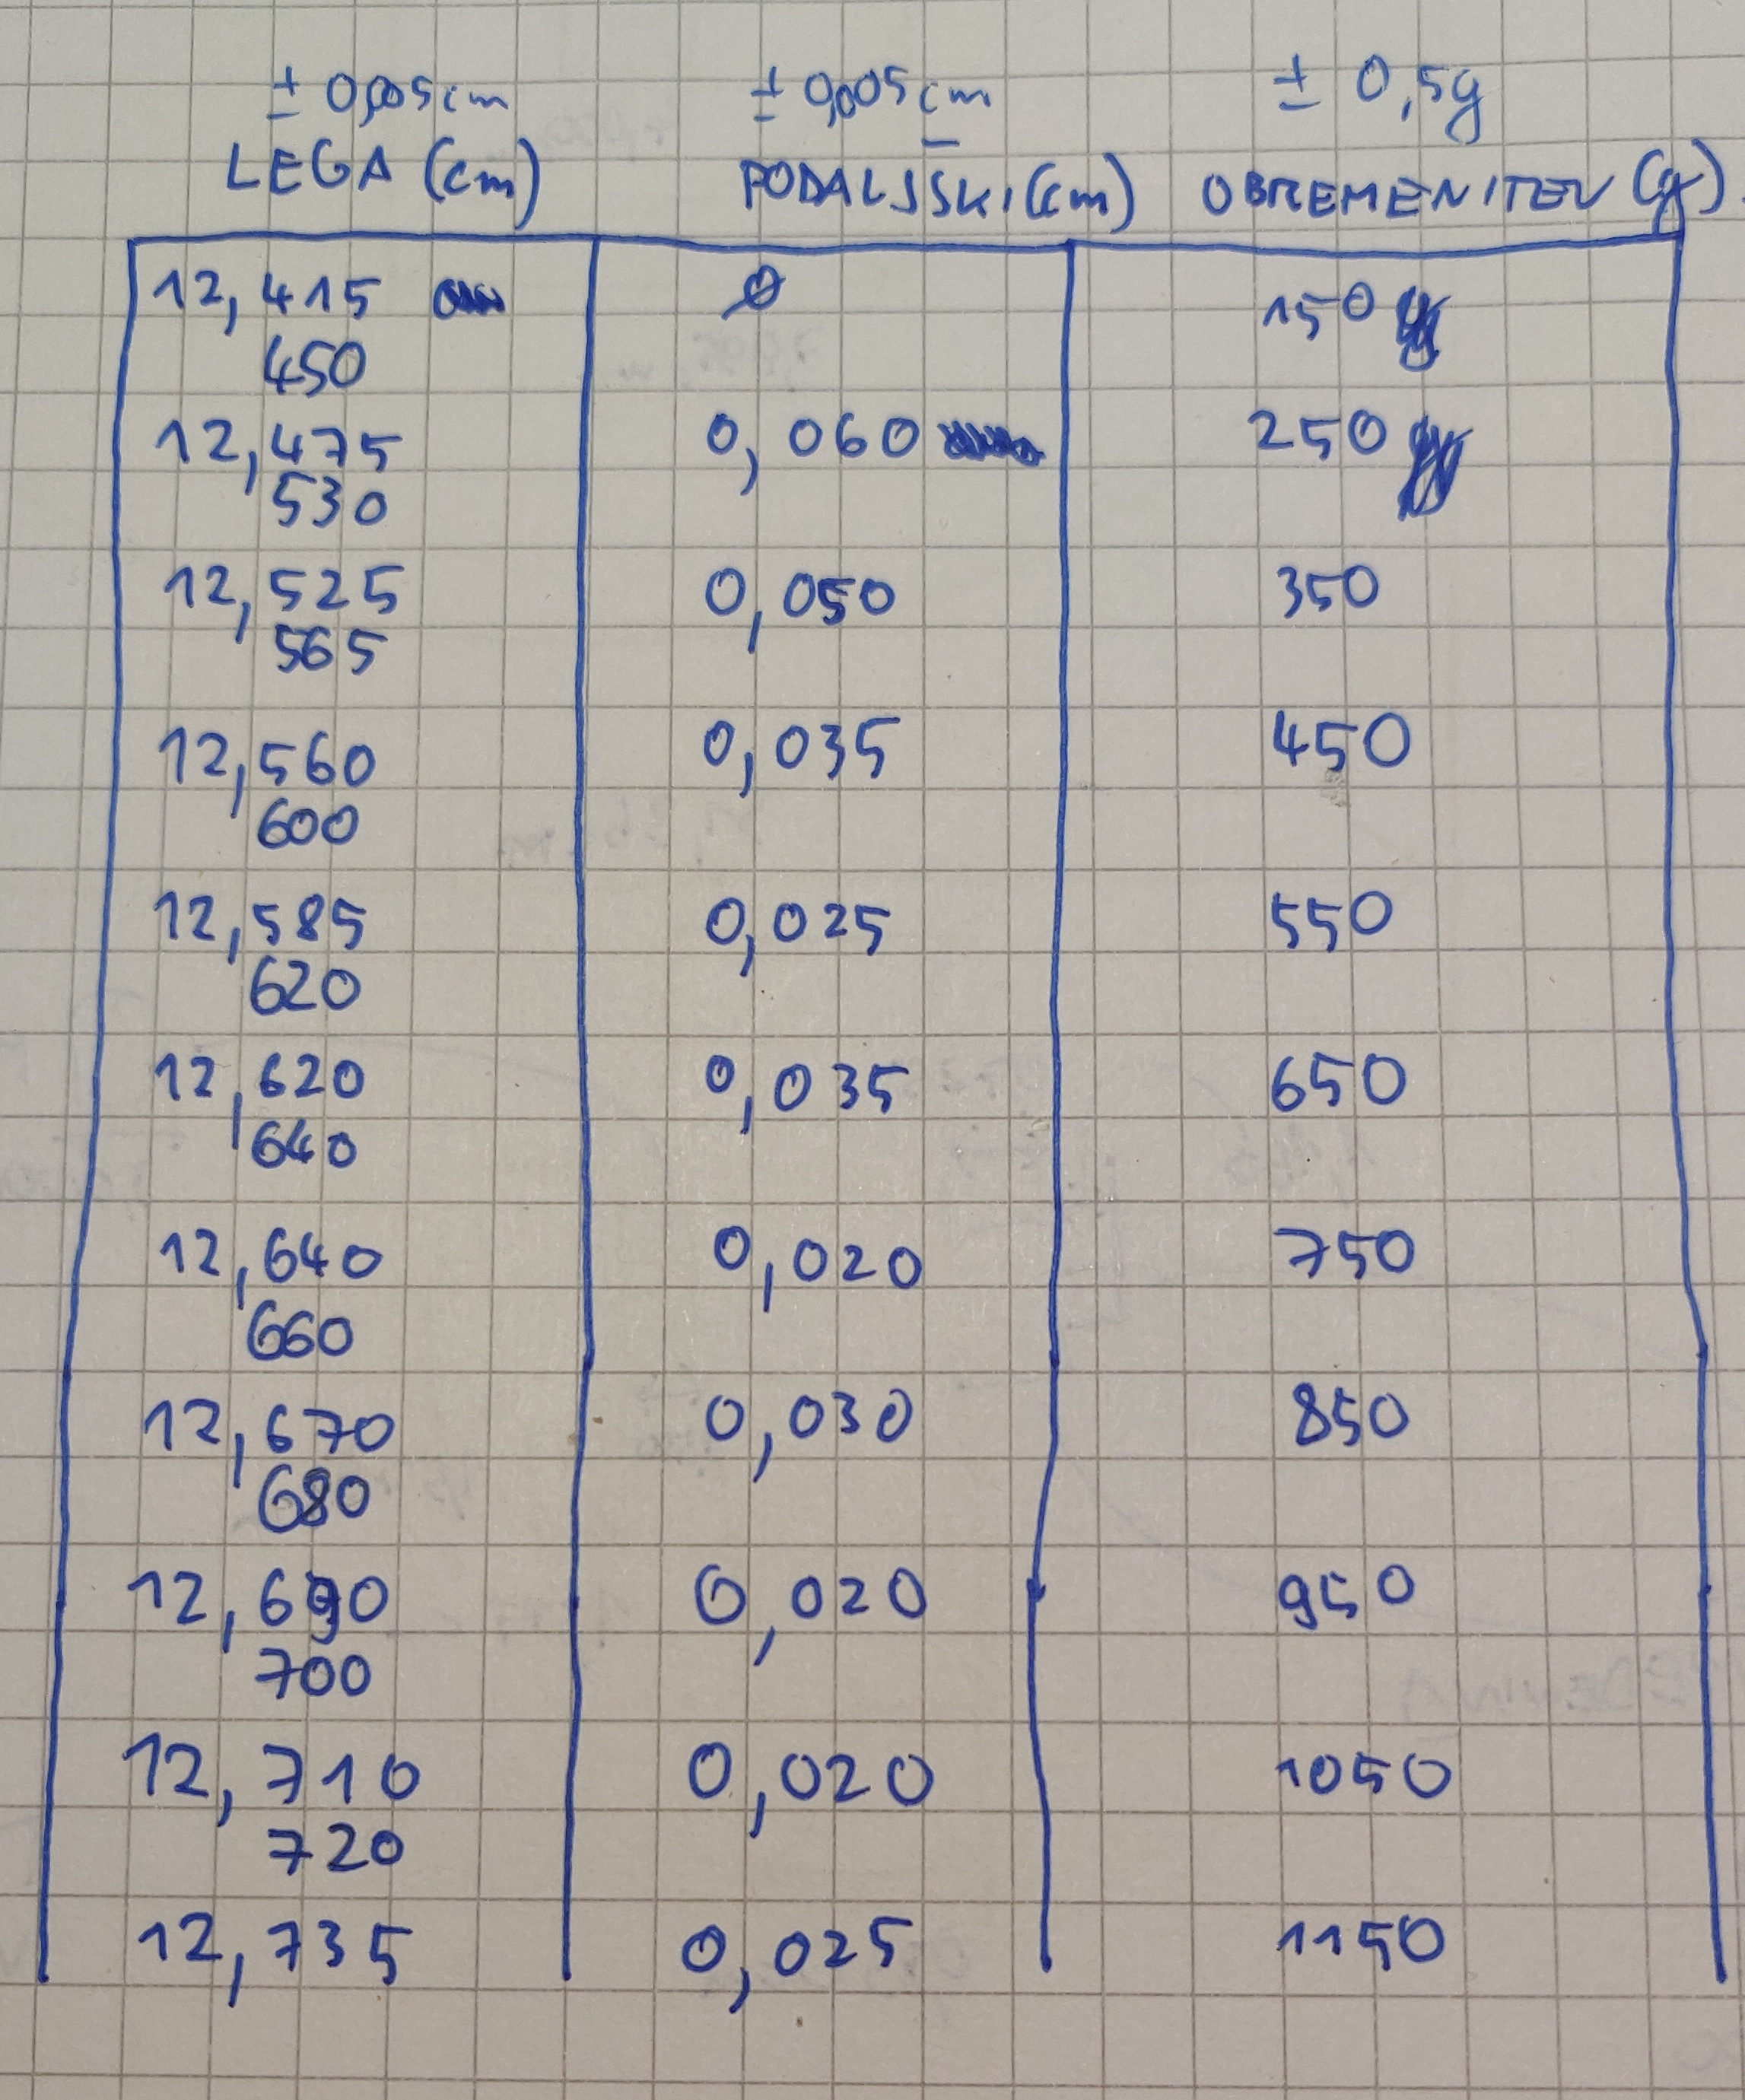
\includegraphics[scale=0.08]{jeklo}\\
za jeklo in \\
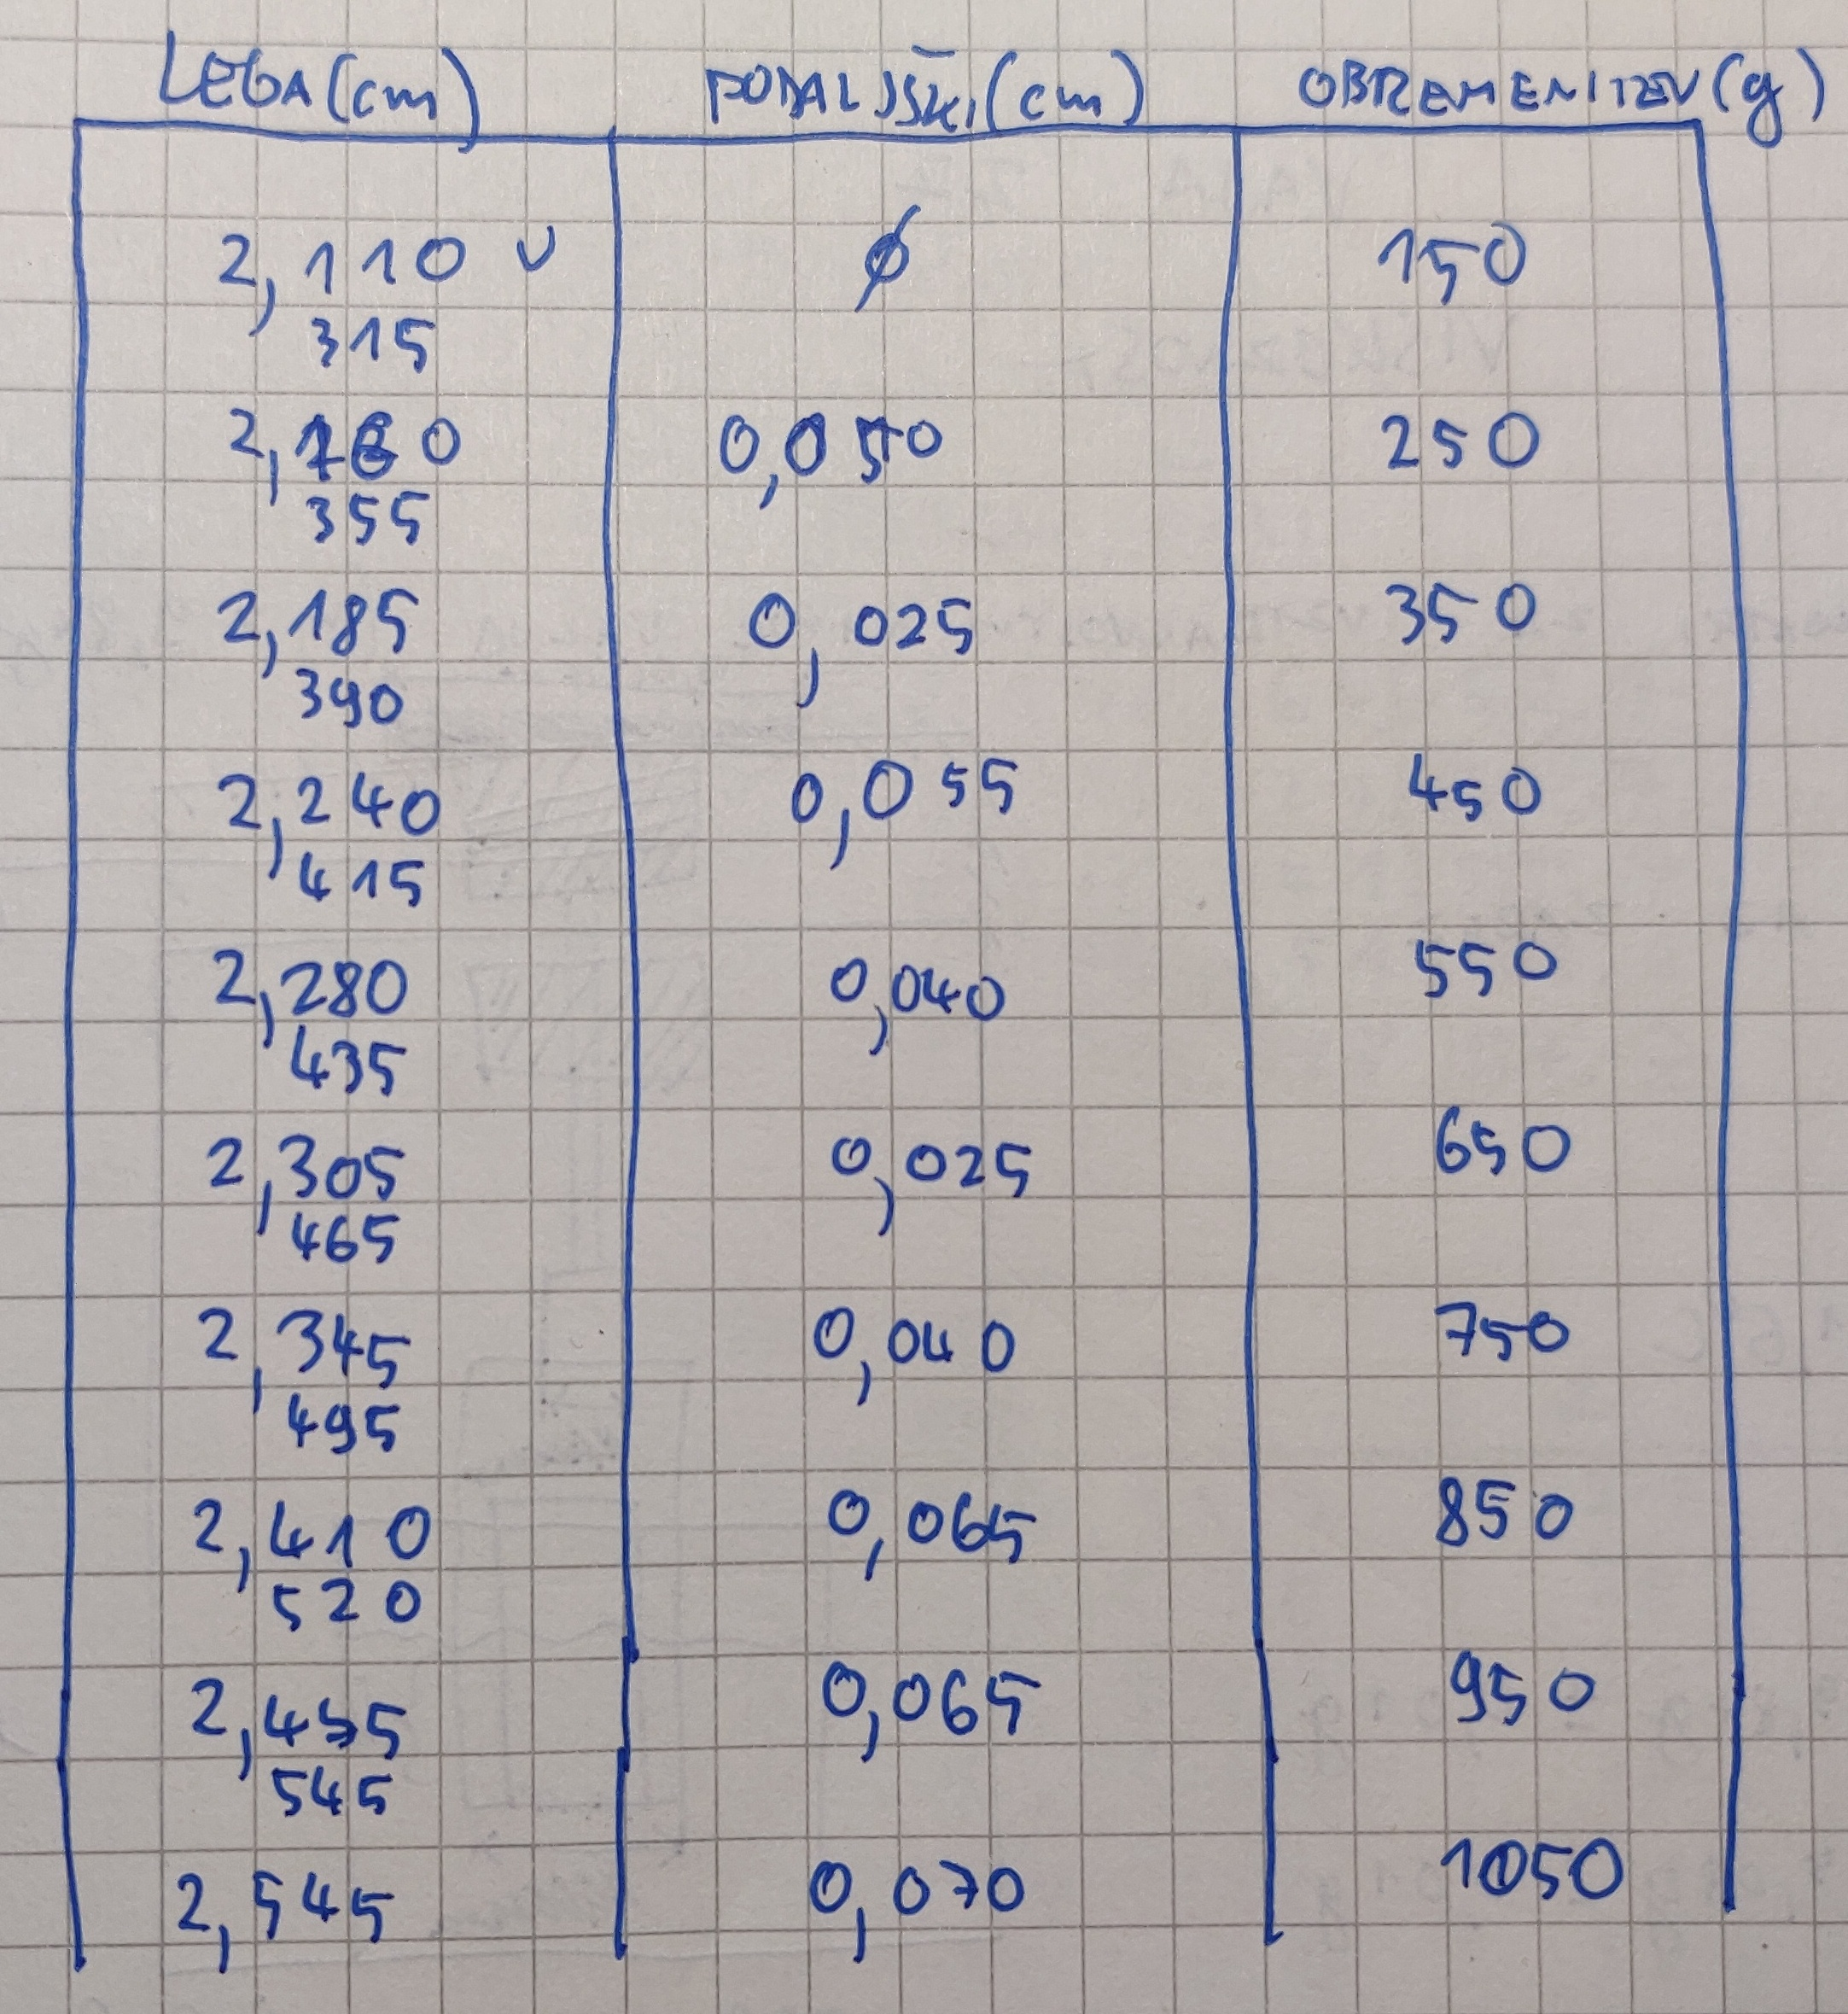
\includegraphics[scale=0.08]{baker}\\
za baker.
\chapter*{Računi}
\section*{Prožnostni modul}
Iz enačbe
\[E=\frac{1}{k}\]
in $k$  pridobljenega iz grafa lahko izračunamo prožnostni modul jeklene in bakrene žice.\\
Za baker tako dobimo
\[E_{baker}=4,6\cdot 10^6\cdot(1\pm0,12)N/cm^2\]
za jeklo pa
\[E_{jeklo}=1,1\cdot 10^7\cdot(1\pm0,15)N/cm^2\]
\section*{Meja linearnosti}
Iz tabele preberemo, da raztezki pri bakru začno naraščati pri obremenitvi 850g. Prav tako je to razvidno iz grafa.\\
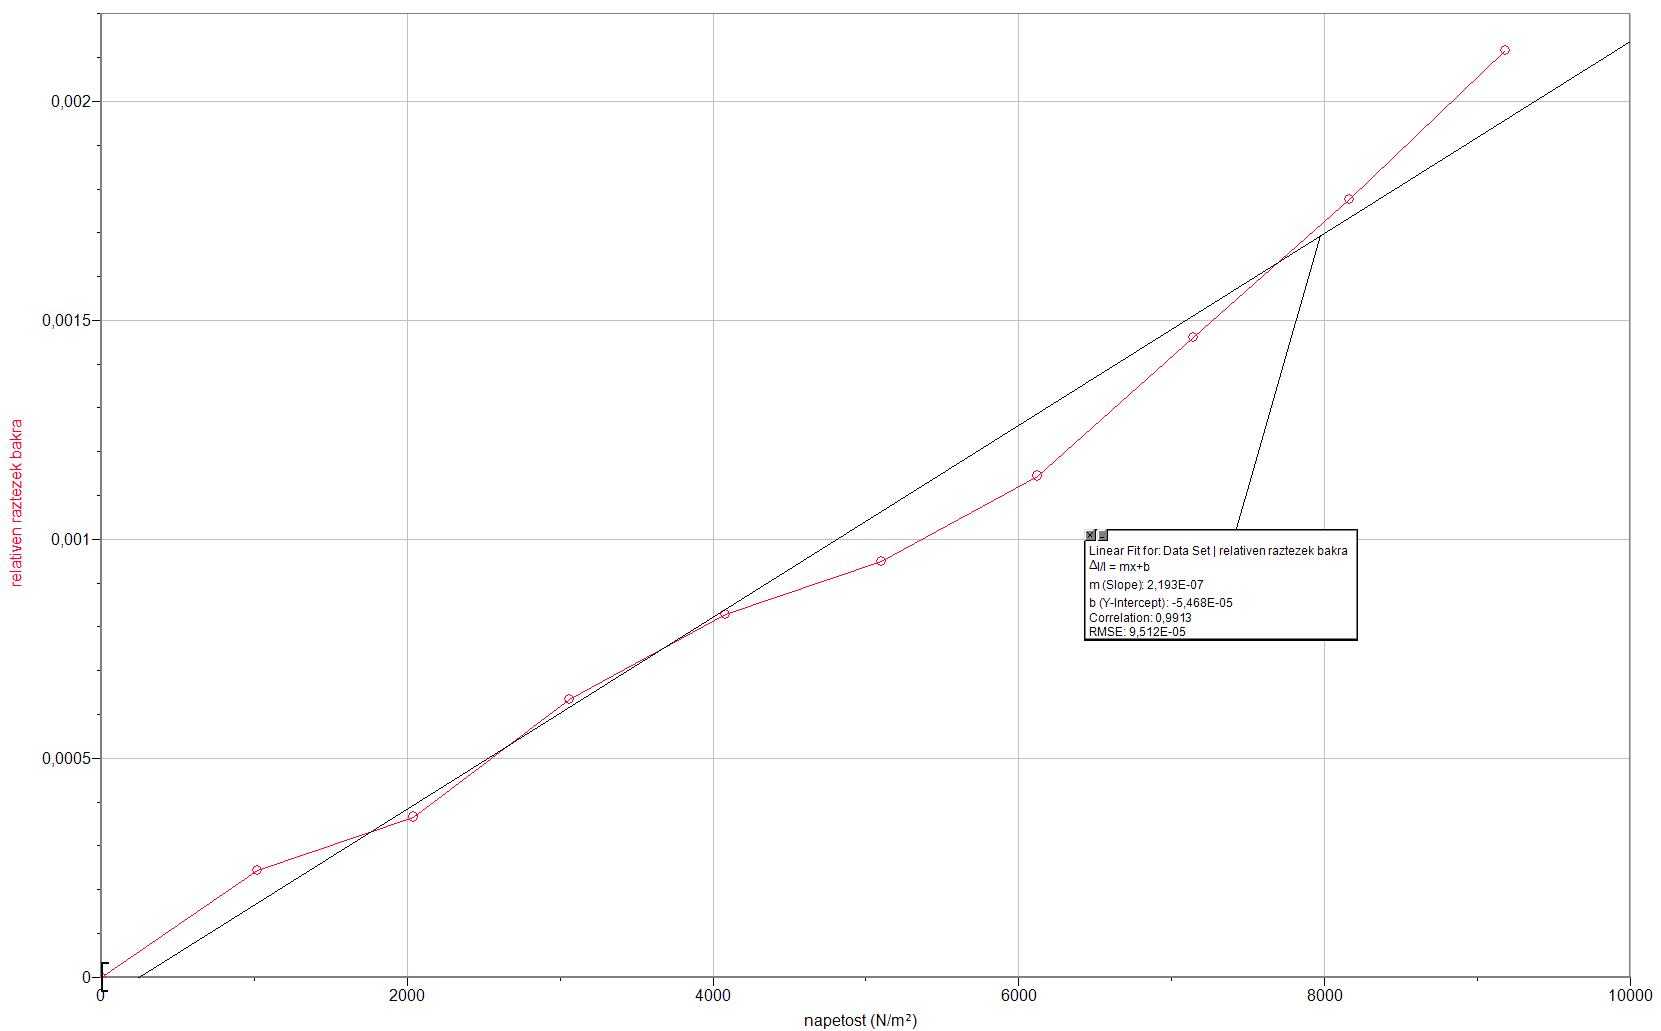
\includegraphics[width=\textwidth]{baker graf}\\
Iz teh podatkov lahko po enačbi za napetost izračunamo mejo linearnosti.

\[\frac{F}{S}=\frac{mg}{(\frac{d}{2})^2\pi}=\frac{0,850kg\cdot 9,81 m/s^2}{14^2\cdot 10^{-10}m^2\cdot\pi}=1,4\cdot 10^{4}\cdot(1\pm0,12)N/cm^2\]

\section*{Natezna trdnosti}
Iz izmerjenih obremenitev ob strgu bakrene žice s premerom 0,12mm\\

\begin{center}
\begin{tabular}{| c | c |}
\hline
Meritev & Obremenitev [g]\\
\hline
1. & 240\\
2. & 240\\
3. & 240\\
4. & 250\\
5. & 250\\ \hline
\end{tabular}\\
\end{center}
\noindent izračunamo povprečno obremenitev ob strgu
\[\overline{m}=244g \pm 5g \]
Iz te pa nato izračunamo mejo natezne trdnosti kot:
\[\frac{F}{S}=\frac{\overline{m}g}{(\frac{d}{2})^2\pi}=\frac{0,244(1\pm0,02)kg\cdot 9,81 m/s^2}{36\cdot 10^{-10}m^2\cdot\pi}=2,1\cdot 10^{4}\cdot(1\pm0,02)N/cm^2\]


\end{document}